
%%--------------------------------------------------
%% Serway: Physics for Scientists and Engineers
%%--------------------------------------------------


%% Chapter 15: Oscillatory Motion
%%--------------------------------------------------


%% Table of Contents
%%--------------------------------------------------

%% 15.1 Motion of an Object Attached to a Spring
%% 15.2 The Particle in Simple Harmonic Motion
%% 15.3 Energy of the Simple Harmonic Oscillator
%% 15.4 Comparing Simple Harmonic Motion with
%% 15.5 Uniform Circular Motion
%% 15.6 The Pendulum
%% 15.7 Damped Oscillations
%% 15.8 Forced Oscillations


%% Serway Multiple Choice Questions
%%--------------------------------------------------
\element{serway-mc}{
\begin{question}{serway-ch15-q01}
    A body of mass \SI{5.0}{\kilo\gram} is suspended by a spring which stretches \SI{10}{\centi\meter} when the mass is attached.
    It is then displaced downward an additional \SI{5.0}{\centi\meter} and released.
    Its position as a function of time is approximately:
    \begin{choices}
        \wrongchoice{$y = 0.10\sin\left(9.9t\right)$}
        \wrongchoice{$y = 0.10\cos\left(9.9t\right)$}
        \wrongchoice{$y = 0.10\cos\left(9.9t + 0.1\right)$}
        \wrongchoice{$y = 0.10\sin\left(9.9t + 5\right)$}
      \correctchoice{$y = 0.05\cos\left(9.9t\right)$}
    \end{choices}
\end{question}
}

\element{serway-mc}{
\begin{question}{serway-ch15-q02}
    A body oscillates with simple harmonic motion along the $x$-axis.
    Its displacement varies with time according to the equation $x=5.0\sin\left(\pi t\right)$.
    The acceleration of the body at $t=\SI{1.0}{\second}$ is approximately:
    \begin{multicols}{3}
    \begin{choices}
        \wrongchoice{\SI{3.5}{\meter\per\second\squared}}
        \wrongchoice{\SI{49}{\meter\per\second\squared}}
        \wrongchoice{\SI{14}{\meter\per\second\squared}}
      \correctchoice{\SI{43}{\meter\per\second\squared}}
        \wrongchoice{\SI{4.3}{\meter\per\second\squared}}
    \end{choices}
    \end{multicols}
\end{question}
}

\element{serway-mc}{
\begin{question}{serway-ch15-q03}
    A body oscillates with simple harmonic motion along the $x$ axis.
    Its displacement varies with time according to the equation
        $x = 5\sin\left(\pi t + \pi/3\right)$.
    The phase of the motion at $t=\SI{2}{\second}$ is:
    \begin{multicols}{3}
    \begin{choices}
      \correctchoice{$\dfrac{7\pi}{3}\,\si{\radian}$}
        \wrongchoice{$\dfrac{\pi}{3}\,\si{\radian}$}
        \wrongchoice{$\pi\,\si{\radian}$}
        \wrongchoice{$\dfrac{5\pi}{3}\,\si{\radian}$}
        \wrongchoice{$2\pi\,\si{\radian}$}
    \end{choices}
    \end{multicols}
\end{question}
}

\element{serway-mc}{
\begin{question}{serway-ch15-q04}
    A body oscillates with simple harmonic motion along the $x$ axis.
    Its displacement varies with time according to the equation
        $x = 5.0\sin\left(\pi t + \pi/3\right)$.
    The velocity of the body at $t=\SI{1.0}{\second}$ is:
    \begin{multicols}{2}
    \begin{choices}
        \wrongchoice{\SI{+8.0}{\meter\per\second}}
      \correctchoice{\SI{-8.0}{\meter\per\second}}
        \wrongchoice{\SI{-14}{\meter\per\second}}
        \wrongchoice{\SI{+14}{\meter\per\second}}
        \wrongchoice{\SI{-5.0}{\meter\per\second}}
    \end{choices}
    \end{multicols}
\end{question}
}

\element{serway-mc}{
\begin{question}{serway-ch15-q05}
    The motion of a particle connected to a spring is described by $x=10\sin\left(\pi t\right)$.
    At what time is the potential energy equal to the kinetic energy?
    \begin{multicols}{3}
    \begin{choices}
        \wrongchoice{zero}
      \correctchoice{\SI{0.25}{\second}}
        \wrongchoice{\SI{0.50}{\second}}
        \wrongchoice{\SI{0.79}{\second}}
        \wrongchoice{\SI{1.0}{\second}}
    \end{choices}
    \end{multicols}
\end{question}
}

\element{serway-mc}{
\begin{question}{serway-ch15-q06}
    The amplitude of a system moving with simple harmonic motion is doubled.
    The total energy will then be:
    \begin{choices}
      \correctchoice{4 times larger}
        \wrongchoice{3 times larger}
        \wrongchoice{2 times larger}
        \wrongchoice{the same as it was}
        \wrongchoice{half as much}
    \end{choices}
\end{question}
}

\element{serway-mc}{
\begin{question}{serway-ch15-q07}
    A mass $m=\SI{2.0}{\kilo\gram}$ is attached to a spring having a force constant $k=\SI{290}{\newton\per\meter}$ as in the figure.
    \begin{center}
    \begin{tikzpicture}
        %% NOTE: TODO: draw tikz
    \end{tikzpicture}
    \end{center}
    The mass is displaced from its equilibrium position and released.
    Its frequency of oscillation is approximately:
    \begin{multicols}{3}
    \begin{choices}
        \wrongchoice{\SI{12}{\hertz}}
        \wrongchoice{\SI{0.50}{\hertz}}
        \wrongchoice{\SI{0.01}{\hertz}}
      \correctchoice{\SI{1.9}{\hertz}}
        \wrongchoice{\SI{0.08}{\hertz}}
    \end{choices}
    \end{multicols}
\end{question}
}

\element{serway-mc}{
\begin{question}{serway-ch15-q08}
    The mass in the figure slides on a frictionless surface.
    \begin{center}
    \begin{tikzpicture}
        %% NOTE: TODO: draw tikz
    \end{tikzpicture}
    \end{center}
    If $m=\SI{2}{\kilo\gram}$, $k_1=\SI{800}{\newton\per\meter}$ and $k_2=\SI{500}{\newton\per\meter}$,
        the frequency of oscillation is approximately:
    \begin{multicols}{3}
    \begin{choices}
        \wrongchoice{\SI{6}{\hertz}}
        \wrongchoice{\SI{2}{\hertz}}
      \correctchoice{\SI{4}{\hertz}}
        \wrongchoice{\SI{8}{\hertz}}
        \wrongchoice{\SI{10}{\hertz}}
    \end{choices}
    \end{multicols}
\end{question}
}

\element{serway-mc}{
\begin{question}{serway-ch15-q09}
    Two circus clowns (each having a mass of \SI{50}{\kilo\gram})
        swing on two flying trapezes (negligible mass, length \SI{25}{\meter})
        shown in the figure.
    \begin{center}
    \begin{tikzpicture}
        %% NOTE: TODO: draw tikz
    \end{tikzpicture}
    \end{center}
    At the peak of the swing, one grabs the other,
        and the two swing back to one platform.
    The time for the forward and return motion is:
    \begin{multicols}{3}
    \begin{choices}
      \correctchoice{\SI{10}{\second}}
        \wrongchoice{\SI{50}{\second}}
        \wrongchoice{\SI{15}{\second}}
        \wrongchoice{\SI{20}{\second}}
        \wrongchoice{\SI{25}{\second}}
    \end{choices}
    \end{multicols}
\end{question}
}

\element{serway-mc}{
\begin{question}{serway-ch15-q10}
    A uniform rod (mass $m=\SI{1.0}{\kilo\gram}$ and length $L=\SI{2.0}{\meter}$) pivoted at one end oscillates in a vertical plane as shown below.
    \begin{center}
    \begin{tikzpicture}
        %% NOTE: TODO: draw tikz
    \end{tikzpicture}
    \end{center}
    The period of oscillation is approximately:
    \begin{multicols}{3}
    \begin{choices}
        \wrongchoice{\SI{4.0}{\second}}
        \wrongchoice{\SI{1.6}{\second}}
        \wrongchoice{\SI{3.2}{\second}}
      \correctchoice{\SI{2.3}{\second}}
        \wrongchoice{\SI{2.0}{\second}}
    \end{choices}
    \end{multicols}
\end{question}
}

\element{serway-mc}{
\begin{question}{serway-ch15-q11}
    A horizontal plank ($m=\SI{2.0}{\kilo\gram}$, $L=\SI{1.0}{\meter}$) is pivoted at one end.
    A spring ($k=\SI{1.0e3}{\newton\per\meter}$) is attached at the other end,
        as shown in the figure.
    \begin{center}
    \begin{tikzpicture}
        %% NOTE: TODO: draw tikz
    \end{tikzpicture}
    \end{center}
    Find the angular frequency for small oscillations.
    \begin{multicols}{2}
    \begin{choices}
      \correctchoice{\SI{39}{\radian\per\second}}
        \wrongchoice{\SI{44}{\radian\per\second}}
        \wrongchoice{\SI{55}{\radian\per\second}}
        \wrongchoice{\SI{66}{\radian\per\second}}
        \wrongchoice{\SI{25}{\radian\per\second}}
    \end{choices}
    \end{multicols}
\end{question}
}

\element{serway-mc}{
\begin{question}{serway-ch15-q12}
    The figure shows a uniform rod (length $L=\SI{1.0}{\meter}$, mass $m=\SI{2.0}{\kilo\gram}$) suspended from a pivot a distance $d=\SI{0.25}{\meter}$ above its center of mass.
    \begin{center}
    \begin{tikzpicture}
        %% NOTE: TODO: draw tikz
    \end{tikzpicture}
    \end{center}
    The angular frequency for small oscillations is approximately axis:
    \begin{multicols}{3}
    \begin{choices}
        \wrongchoice{\SI{1.0}{\radian\per\second}}
        \wrongchoice{\SI{2.5}{\radian\per\second}}
        \wrongchoice{\SI{1.5}{\radian\per\second}}
      \correctchoice{\SI{4.1}{\radian\per\second}}
        \wrongchoice{\SI{3.5}{\radian\per\second}}
    \end{choices}
    \end{multicols}
\end{question}
}

\element{serway-mc}{
\begin{question}{serway-ch15-q13}
    In the figure below, a disk (radius $R=\SI{1.0}{\meter}$, mass $m=\SI{2.0}{\kilo\gram}$) is suspended from a pivot a distance $d=\SI{0.25}{\meter}$ above its center of mass.
    \begin{center}
    \begin{tikzpicture}
        %% NOTE: TODO: draw tikz
    \end{tikzpicture}
    \end{center}
    The angular frequency for small oscillations is approximately axis:
    \begin{multicols}{2}
    \begin{choices}
        \wrongchoice{\SI{4.2}{\radian\per\second}}
      \correctchoice{\SI{2.1}{\radian\per\second}}
        \wrongchoice{\SI{1.5}{\radian\per\second}}
        \wrongchoice{\SI{1.0}{\radian\per\second}}
        \wrongchoice{\SI{3.8}{\radian\per\second}}
    \end{choices}
    \end{multicols}
\end{question}
}

\element{serway-mc}{
\begin{question}{serway-ch15-q14}
    In the figure below, a hoop (radius $R=\SI{1.0}{\meter}$, mass  $m=\SI{2.0}{\kilo\gram}$) having four spokes of negligible mass is suspended from a pivot a distance $d=\SI{0.25}{\meter}$ above its center of mass.
    \begin{center}
    \begin{tikzpicture}
        %% NOTE: TODO: draw tikz
    \end{tikzpicture}
    \end{center}
    The angular frequency for small oscillations is approximately axis:
    \begin{multicols}{3}
    \begin{choices}
        \wrongchoice{\SI{4.0}{\radian\per\second}}
        \wrongchoice{\SI{2.5}{\radian\per\second}}
      \correctchoice{\SI{1.5}{\radian\per\second}}
        \wrongchoice{\SI{1.0}{\radian\per\second}}
        \wrongchoice{\SI{0.5}{\radian\per\second}}
    \end{choices}
    \end{multicols}
\end{question}
}

\element{serway-mc}{
\begin{question}{serway-ch15-q15}
    A torsional pendulum consists of a solid disk (mass $m=\SI{2.0}{\kilo\gram}$, radius $R=\SI{1.0}{\meter}$) suspended by a wire attached to a rigid support.
    \begin{center}
    \begin{tikzpicture}
        %% NOTE: TODO: draw tikz
    \end{tikzpicture}
    \end{center}
    The body oscillates about the support wire.
    If the torsion constant is \SI{16}{\newton\meter}.
    What is the angular frequency?
    \begin{multicols}{3}
    \begin{choices}
        \wrongchoice{\SI{2}{\radian\per\second}}
      \correctchoice{\SI{4}{\radian\per\second}}
        \wrongchoice{\SI{6}{\radian\per\second}}
        \wrongchoice{\SI{8}{\radian\per\second}}
        \wrongchoice{\SI{7}{\radian\per\second}}
    \end{choices}
    \end{multicols}
\end{question}
}

\element{serway-mc}{
\begin{question}{serway-ch15-q16}
    The mass in the figure below slides on a frictionless surface.
    \begin{center}
    \begin{tikzpicture}
        %% NOTE: TODO: draw tikz
    \end{tikzpicture}
    \end{center}
    When the mass is pulled out,
        spring 1 is stretched a distance $x_1$ from its equilibrium position and spring 2 is stretched a distance $x_2$.
    The spring constants are $k_1$ and $k_2$ respectively.
    The force pulling back on the mass is:
    \begin{multicols}{2}
    \begin{choices}
        \wrongchoice{$-k_2 x_1$}
      \correctchoice{$-k_2 x_2$}
        \wrongchoice{$-\left(k_1 x_1 + k_2 x_2\right)$}
        \wrongchoice{$-\dfrac{k_1+k_2}{2}\left(x_1 + x_2\right)$}
        \wrongchoice{$-\dfrac{k_1+k_2}{k_1 k_2}\left(x_1 + x_2\right)$}
    \end{choices}
    \end{multicols}
\end{question}
}

\element{serway-mc}{
\begin{question}{serway-ch15-q17}
    A hoop, a solid cylinder, and a solid sphere all have the same mass $m$ and the same radius $R$.
    Each is mounted to oscillate about an axis a distance $0.5 R$ from the center.
    The axis is perpendicular to the circular plane of the hoop and the cylinder and to an equatorial plane of the sphere as shown below.
    \begin{center}
    \begin{tikzpicture}
        %% NOTE: TODO: draw tikz
    \end{tikzpicture}
    \end{center}
    Which is the correct ranking in order of increasing angular frequency $\omega$?
    \begin{choices}
      \correctchoice{hoop, cylinder, sphere}
        \wrongchoice{cylinder, sphere, hoop}
        \wrongchoice{sphere, cylinder, hoop}
        \wrongchoice{hoop, sphere, cylinder}
        \wrongchoice{sphere, hoop, cylinder}
    \end{choices}
\end{question}
}

\element{serway-mc}{
\begin{question}{serway-ch15-q18}
    Three pendulums with strings of the same length and bobs of the same mass are pulled out to angles $\theta_1$, $\theta_2$ and $\theta_3$ respectively and released.
    The approximation $\sin\theta=\theta$ holds for all three angles,
        with $\theta_3 > \theta_2 > \theta_1$.
    How do the angular frequencies of the three pendulums compare?
    \begin{choices}
        \wrongchoice{$\omega_3 > \omega_2 > \omega_1$}
        \wrongchoice{Need to know amplitudes to answer this question.}
        \wrongchoice{Need to know $\sqrt{g/L}$ to answer this question.}
        \wrongchoice{$\omega_1 > \omega_2 > \omega_3$}
      \correctchoice{$\omega_1 = \omega_2 = \omega_3$}
    \end{choices}
\end{question}
}

\element{serway-mc}{
\begin{question}{serway-ch15-q19}
    A weight of mass $m$ is at rest at $O$ when suspended from a spring, as shown.
    \begin{center}
    \begin{tikzpicture}
        %% NOTE: TODO: draw tikz
    \end{tikzpicture}
    \end{center}
    When it is pulled down and released,
        it oscillates between positions $A$ and $B$.
    Which statement about the system consisting of the spring and the mass is correct?
    \begin{choices}
        \wrongchoice{The gravitational potential energy of the system is greatest at $A$.}
        \wrongchoice{The elastic potential energy of the system is greatest at $O$.}
      \correctchoice{The rate of change of momentum has its greatest magnitude at $A$ and $B$.}
        \wrongchoice{The rate of change of gravitational potential energy is smallest at $O$.}
        \wrongchoice{The rate of change of gravitational potential energy has its greatest magnitude at $A$ and $B$.}
    \end{choices}
\end{question}
}

\element{serway-mc}{
\begin{questionmult}{serway-ch15-q20}
    An object of mass $m$ is attached to string of length $L$.
    When it is released from point $A$,
        the object oscillates between points $A$ and $B$.
    \begin{center}
    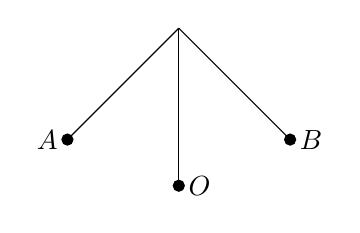
\begin{tikzpicture}
        \draw (0,0) -- (315:2);
        \draw[fill] (315:2) circle (2pt) node[anchor=west] {$B$};
        \draw (0,0) -- (270:2);
        \draw[fill] (270:2) circle (2pt) node[anchor=west] {$O$};
        \draw (0,0) -- (225:2);
        \draw[fill] (225:2) circle (2pt) node[anchor=east] {$A$};
    \end{tikzpicture}
    \end{center}
    Which statement about the system consisting of the pendulum and the Earth is correct?
    \begin{choices}
      \correctchoice{The gravitational potential energy of the system is greatest at $A$ and $B$.}
      \correctchoice{The kinetic energy of mass $m$ is greatest at point $O$.}
      \correctchoice{The greatest rate of change of momentum occurs at $A$ and $B$.}
        %\wrongchoice{All of the above are correct.}
        %\wrongchoice{Only (a) and (b) above are correct.}
    \end{choices}
\end{questionmult}
}

\newcommand{\serwayChFifteenQTwentyOne}{
\begin{tikzpicture}
    %% NOTE: TODO: draw tikz
\end{tikzpicture}
}

\element{serway-mc}{
\begin{question}{serway-ch15-q21}
    A graph of position versus time for an object oscillating at the free end of a horizontal spring is shown below.
    \begin{center}
        \serwayChFifteenQTwentyOne
    \end{center}
    A point or points at which the object has positive velocity and zero acceleration is(are):
    %% NOTE: Question mult
    \begin{multicols}{3}
    \begin{choices}
        \wrongchoice{$B$}
        \wrongchoice{$C$}
        \wrongchoice{$D$}
        \wrongchoice{$B$ or $D$}
      \correctchoice{$A$ or $E$}
    \end{choices}
    \end{multicols}
\end{question}
}

\element{serway-mc}{
\begin{question}{serway-ch15-q22}
    A graph of position versus time for an object oscillating at the free end of a horizontal spring is shown below.
    \begin{center}
        \serwayChFifteenQTwentyOne
    \end{center}
    The point at which the object has negative velocity and zero acceleration is
    \begin{multicols}{3}
    \begin{choices}[o]
        \wrongchoice{$A$}
        \wrongchoice{$B$}
      \correctchoice{$C$}
        \wrongchoice{$D$}
        \wrongchoice{$E$}
    \end{choices}
    \end{multicols}
\end{question}
}

\element{serway-mc}{
\begin{question}{serway-ch15-q23}
    A graph of position versus time for an object oscillating at the free end of a horizontal spring is shown below.
    \begin{center}
        \serwayChFifteenQTwentyOne
    \end{center}
    The point at which the object has zero velocity and positive acceleration is:
    \begin{multicols}{3}
    \begin{choices}[o]
        \wrongchoice{$A$}
        \wrongchoice{$B$}
        \wrongchoice{$C$}
      \correctchoice{$D$}
        \wrongchoice{$E$}
    \end{choices}
    \end{multicols}
\end{question}
}

\element{serway-mc}{
\begin{question}{serway-ch15-q24}
    A graph of position versus time for an object oscillating at the free end of a horizontal spring is shown below.
    \begin{center}
        \serwayChFifteenQTwentyOne
    \end{center}
    The point at which the object has zero velocity and negative acceleration is:
    \begin{multicols}{3}
    \begin{choices}[o]
        \wrongchoice{$A$}
      \correctchoice{$B$}
        \wrongchoice{$C$}
        \wrongchoice{$D$}
        \wrongchoice{$E$}
    \end{choices}
    \end{multicols}
\end{question}
}

\element{serway-mc}{
\begin{question}{serway-ch15-q25}
    In an inertia balance, a body supported against gravity executes simple harmonic oscillations in a horizontal plane under the action of a set of springs.
    If a \SI{1.00}{\kilo\gram} body vibrates at \SI{1.00}{\hertz},
        a \SI{2.00}{\kilo\gram} body will vibrate at:
    \begin{multicols}{2}
    \begin{choices}
        \wrongchoice{\SI{0.500}{\hertz}}
      \correctchoice{\SI{0.707}{\hertz}}
        \wrongchoice{\SI{1.00}{\hertz}}
        \wrongchoice{\SI{1.41}{\hertz}}
        \wrongchoice{\SI{2.00}{\hertz}}
    \end{choices}
    \end{multicols}
\end{question}
}

\element{serway-mc}{
\begin{question}{serway-ch15-q26}
    At sea level, at a latitude where $g=\SI{9.80}{\meter\per\second\squared}$,
        a pendulum that takes \SI{2.00}{\second} for a complete swing back and forth has a length of \SI{0.993}{\meter}.
    What is the value of $g$ at a location where the length of such a pendulum is \SI{0.970}{\meter}?
    \begin{multicols}{2}
    \begin{choices}
        \wrongchoice{\SI{0.0983}{\meter\per\second\squared}}
        \wrongchoice{\SI{3.05}{\meter\per\second\squared}}
      \correctchoice{\SI{9.28}{\meter\per\second\squared}}
        \wrongchoice{\SI{10.0}{\meter\per\second\squared}}
        \wrongchoice{\SI{38.3}{\meter\per\second\squared}}
    \end{choices}
    \end{multicols}
\end{question}
}

\element{serway-mc}{
\begin{question}{serway-ch15-q27}
    Suppose it were possible to drill a frictionless cylindrical channel along a diameter of the Earth from one side of the Earth to another.
    A body dropped into such a channel will only feel the gravitational pull of mass within a sphere of radius equal to the distance of the mass from the center of the Earth .
    The density of the Earth is \SI{5.52e3}{\kilo\gram\per\meter\cubed} and $G=\SI{6.67e-11}{\newton\meter\squared\per\kilo\gram\squared}$.
    The mass will oscillate with a period of:
    \begin{multicols}{3}
    \begin{choices}
      \correctchoice{\SI{84.4}{\minute}}
        \wrongchoice{\SI{169}{\minute}}
        \wrongchoice{\SI{24.0}{\hour}}
        \wrongchoice{\SI{1130}{\hour}}
        \wrongchoice{\SI{27.2}{\day}}
    \end{choices}
    \end{multicols}
\end{question}
}

\element{serway-mc}{
\begin{question}{serway-ch15-q28}
    A \SI{2.00}{\meter} long \SI{6.00}{\kilo\gram} ladder pivoted at the top hangs down from a platform at the circus.
    A \SI{42.0}{\kilo\gram} trapeze artist climbs to a point where her center of mass is at the center of the ladder and swings at the systems natural frequency.
    The angular frequency of the system of ladder and woman is:
    \begin{multicols}{3}
    \begin{choices}
        \wrongchoice{\SI{1.01}{\per\second}}
        \wrongchoice{\SI{2.01}{\per\second}}
      \correctchoice{\SI{4.03}{\per\second}}
        \wrongchoice{\SI{8.05}{\per\second}}
        \wrongchoice{\SI{16.2}{\per\second}}
    \end{choices}
    \end{multicols}
\end{question}
}

\element{serway-mc}{
\begin{question}{serway-ch15-q29}
    Ellen says that whenever the acceleration is directly proportional to the displacement of an object from its equilibrium position,
        the motion of the object is simple harmonic motion. 
    Mary says this is true only if the acceleration is opposite in direction to the displacement. 
    Which one, if either, is correct?
    \begin{choices}
        \wrongchoice{Ellen, because $\omega^2$ is directly proportional to the constant multiplying the displacement and to the mass.}
        \wrongchoice{Ellen, because $\omega^2$ is directly proportional to the mass.}
        \wrongchoice{Mary, because $\omega^2$ is directly proportional to the constant multiplying the displacement and to the mass.}
        \wrongchoice{Mary, because $\omega^2$ is directly proportional to the mass.}
      \correctchoice{Mary, because the second derivative of an oscillatory function like $\sin\left(\omega t\right)$ or $\cos\left(\omega t\right)$ always is the negative of the original function.}
    \end{choices}
\end{question}
}

\element{serway-mc}{
\begin{question}{serway-ch15-q30}
    John says that the value of the function $\cos\left[\omega\left(t+T\right)+\phi\right]$,
    obtained one period $T$ after time $t$, is greater than $\cos\left(\omega t+\phi\right)$ by $2\pi$.
    Larry says that it is greater by the addition of \num{1.00} to $\cos\left(\omega t+\phi\right)$.
    Which one, if either, is correct?
    \begin{choices}
        \wrongchoice{John, because $\omega T = 2\pi$.}
        \wrongchoice{John, because $\omega T = \SI{1}{\radian}$.}
        \wrongchoice{Larry, because $\omega T = 2\pi$ .}
        \wrongchoice{Larry, because $\omega T = \SI{1}{\radian}$.}
      \correctchoice{Neither, because $\cos\left(\theta+2\pi\right)=\cos\theta$.}
    \end{choices}
\end{question}
}

\element{serway-mc}{
\begin{question}{serway-ch15-q31}
    Simple harmonic oscillations can be modeled by the projection of circular motion at constant angular velocity onto a diameter of the circle. 
    When this is done,
        the analog along the diameter of the centripetal acceleration of the particle executing circular motion is:
    \begin{choices}
        \wrongchoice{the displacement from the center of the diameter of the projection of the position of the particle on the circle.}
        \wrongchoice{the projection along the diameter of the velocity of the particle on the circle.}
        \wrongchoice{the projection along the diameter of tangential acceleration of the particle on the circle.}
      \correctchoice{the projection along the diameter of centripetal acceleration of the particle on the circle.}
        \wrongchoice{meaningful only when the particle moving in the circle also has a non-zero tangential acceleration.}
    \end{choices}
\end{question}
}

\element{serway-mc}{
\begin{question}{serway-ch15-q32}
    When a damping force is applied to a simple harmonic oscillator which has angular frequency $\omega_0$ in the absence of damping,
        the new angular frequency $\omega$ is such that:
    \begin{multicols}{2}
    \begin{choices}
      \correctchoice{$\omega < \omega_0$}
        \wrongchoice{$\omega = \omega_0$}
        \wrongchoice{$\omega > \omega_0$}
        \wrongchoice{$\omega T < \omega_0 T_0$}
        \wrongchoice{$\omega T > \omega_0 T_0$}
    \end{choices}
    \end{multicols}
\end{question}
}

\element{serway-mc}{
\begin{question}{serway-ch15-q33}
    When a damping force is applied to a simple harmonic oscillator which has period $T_0$ in the absence of damping,
        the new period $T$ is such that:
    \begin{multicols}{2}
    \begin{choices}
        \wrongchoice{$T < T_0$}
        \wrongchoice{$T = T_0$}
      \correctchoice{$T > T_0$}
        \wrongchoice{$\omega T < \omega_0 T_0$}
        \wrongchoice{$\omega T > \omega_0 T_0$}
    \end{choices}
    \end{multicols}
\end{question}
}

\element{serway-mc}{
\begin{question}{serway-ch15-q34}
    To double the total energy of a mass oscillating at the end of a spring with amplitude $A$,
        we need to:
    \begin{choices}
        \wrongchoice{increase the angular frequency by $\sqrt{2}$.}
      \correctchoice{increase the amplitude by $\sqrt{2}$.}
        \wrongchoice{increase the amplitude by $2$.}
        \wrongchoice{increase the angular frequency by $2$.}
        \wrongchoice{increase the amplitude by 4 and decrease the angular frequency by $\dfrac{1}{\sqrt{2}}$}
    \end{choices}
\end{question}
}


\endinput


